\textbf{\LARGE osn 6. Криволинейный интеграл, формула Грина.}

$\mathLet ~ \varphi(t), \psi(t)$ непр. на $[a,b]$. 
Если рассматривать $t$ как время, эти функции определяют закон движения по плоскости точки $M$ с координатами 
$x = \varphi(t), y = \psi(t), ~ \alpha < t < \beta$. Множество $\{M\}$ всех точек $M$, координаты $x,y$ которых определяются уравнениями $\varphi(t), \psi(t)$, называется \textbf{простой плоской кривой} $L$, если различным значениям параметра $t$ из $[\alpha, \beta]$ отвечают различные точки этого множества.

$\mathLet ~ \varphi(t), \psi(t) \in C[\{t\}]$. Уравнения $x = \varphi(t), y = \psi(t)$ задают параметрически кривую L, если $\exists$ такая система сегментов $\{[t_{i-1}, t_i]\}$, разбивающих множество $\{t\}$, что для значений $t$ из каждого данного сегмента этой системы все уравнения определяют простую кривую.

\textbf{Спрямляемая кривая} --- кривая, имеющая конечную длину.

\textbf{Длина кривой} -- это предел последовательности длин ломаных, вписанных в эту линию, при условии, что длина наибольшего звена $\rightarrow 0$.

\bigbreak
$\mathLet ~ x = \varphi(t), y = \psi(t) \in C[\alpha, \beta]$. Тогда кривая $L$, определяемая $x, y$, спрямляема и длину $l$ ее дуги можно вычислить по формуле
$$l = \int^{\beta}_{\alpha} \sqrt{\varphi'^2(t) + \psi'^2(t)}dt$$

\faEye \ произвольную спрямляемую кривую $L$ на плоскости $Oxy$, не имеющую точек самопересечения и самоналегания, незамкнутую, ограниченную точками $A,~B$, описывающуюся параметрическими ур-ями:
$$\begin{cases} x=\varphi(t)&\\ y=\psi(t)\end{cases},~t\in [a,b], A=(\varphi(a),\psi(a)), B=(\varphi(b),\psi(b))$$

\mathLet \ на кривой L определены три непрерывные вдоль этой кривой функции $f(x,y)=f(M),~P(x,y)=P(M),~Q(x,y)=Q(M)$.

\faEye \ разбиение отрезка 
$[a,b]:~a=t_0 < t_1 < \dots < t_n = b,~$
$\Delta t_k = t_k-t_{k-1}, ~ M_k = M_k(\varphi(t_k),\psi(t_k))$.

$\Delta l_k = |\smile M_{k-1}M_k|$ (длина дуги), $\Delta \equiv \displaystyle\max_{1\leqslant k\leqslant n} \Delta l_k$.

Выберем точки $N_k(\xi_k, \eta_k) \in \smile M_{k-1}M_k,~\xi_k=\varphi(\tau_k),~\eta_k=\psi(\tau_k),~\tau_k\in [t_{k-1},t_k]$.

$\Delta x_k = x_k - x_{k-1},~x_k = \varphi(t_k),~\Delta y_k = y_k - y_{k-1},~y_k = \psi(t_k)$

\faEye \ три интегральные суммы:
\begin{enumerate}
    \item $\sigma_1=\displaystyle\sum_{k=1}^n f(N_k)\Delta l_k$
    \item $\sigma_2=\displaystyle\sum_{k=1}^n P(N_k)\Delta x_k$
    \item $\sigma_3=\displaystyle\sum_{k=1}^n Q(N_k)\Delta y_k$
\end{enumerate}

Число $I_s,~s=1,2,3$ называется \textbf{пределом интегральной суммы} $\sigma_s$ при $\Delta \rightarrow 0$, если $\forall\varepsilon>0~\exists\delta>0:~\Delta<\delta\implies|I_s-\sigma_s|<\varepsilon$ независимо от выбора точек $N_k\in\smile M_{k-1}M_k$.

Если существует предел $I_1$ интегральной суммы $\sigma_1$ при $\Delta \rightarrow 0$, то он называется \textbf{криволинейным интегралом 1 рода} от функции $f$ по кривой $L$.
$$I_1=\displaystyle\lim_{\Delta\to 0}\sigma_1
= \int\limits_{L}f(x,y)dl 
%=\int\limits_{\smile AB}f(x,y)dl 
=\int\limits_{a}^{b} f(\varphi(t), \psi(t)) \sqrt{ \varphi_t^{'2}(t) + \psi_t^{'2}(t) } dt $$

Если существуют пределы $I_2,~I_3$ интегральных сумм $\sigma_2,~\sigma_3$ при $\Delta \rightarrow 0$, то они называются \textbf{криволинейными интегралами 2} рода от функций $P,~Q$ по кривой $AB$.
$$I_2=\displaystyle\lim_{\Delta\to 0}\sigma_2= \int\limits_{\smile AB}P(x,y)dx =\int\limits_{\smile AB}P(M)dx $$
$$I_3=\displaystyle\lim_{\Delta\to 0}\sigma_3= \int\limits_{\smile AB}Q(x,y)dy =\int\limits_{\smile AB}Q(M)dy $$

$I_2+I_3=\int\limits_{\smile AB}P(x,y)dx+\int\limits_{\smile AB}Q(x,y)dy = \int\limits_{\smile AB}P(x,y)dx+Q(x,y)dy$ 

-- \textbf{общий криволинейный интеграл 2 рода}.

Из определения криволинейных интегралов следует, что:
\begin{enumerate}
    \item криволинейный интеграл первого рода не зависит от того, в каком направлении пробегает кривая $L$, а для криволинейного интеграла второго рода изменение направления кривой ведёт к изменению знака, т.е. $\int\limits_{\smile AB}P(x,y)dx+Q(x,y)dy=-\int\limits_{\smile BA}P(x,y)dx+Q(x,y)dy$
    \item физически криволинейный интеграл первого рода представляет собой массу кривой $L$, линейная плотность которой равна $f(x, y)$;

    общий линейный интеграл второго рода физически представляет собой работу по перемещению материальной точки $A$ в точку $B$ вдоль кривой $L$ под действием силы, имеющей составляющие $P(x, y)$ и $Q(x, y)$.

\end{enumerate}

\todo{Во второй части билета какая-то херня. Закоментированны} \\
\todo{совершенно рандомные куски ибо не влезает. Надо что-то придумать.}

% Область $D$ называется\textbf{ односвязной}, если любая кусочно гладкая замкнутая без самопересечения кривая, расположенная в $D$, ограничивает область, все точки которой также принадлежат $D$.
% $\mathLet ~ \pi$ --- плоскость в пространстве $E_3$, $k$ --- единичный вектор нормали к $\pi$, $D$ --- односвязная область на $\pi$. \mathLet \ далее, область $D$ удовлетворяет следующим условиям:
% \begin{enumerate}
%     \item граница $C$ области $D$ является замкнутой кусочно-гладкой кривой без особых точек;
%     \item на плоскости $\pi$ можно выбрать такую прямоугольную декартову систему координат, что все прямые, параллельные координатным осям, пересекают $C$ не более чем в двух точках.
% \end{enumerate}

$\mathLet ~ t$ --- единичный вектор касательной к кривой $C$, согласованной с $k$, т.е. положительное направление обхода кривой $C$ совпадает в точке приложения вектора $t$ с направлением этого вектора, и если смотреть с конца нормали $k$, то контур $C$ ориентирован положительно (Его обход осуществляется против часовой стрелки). Говорят, что ориентация кривой $C$ согласована с нормалью <<по правилу штопора>>.

\textbf{Опр.} \textbf{Векторным полем} в $\mathcal{R}^3$ называется векторная функция, определенная в $\mathcal{R}^3$ (или на $D \subset \mathcal{R}^3$): $\overline{f}(M): \mathcal{R}^3 \rightarrow \mathcal{R}^3$

\textbf{Опр.} \textbf{Ротором} векторного поля $f(M)$ называется $rot\mathcal{A}$

В Орт-Норм Базисе выражение для $rot(f) = rot(f_x \overline{e}_1 + f_y \overline{e}_2 + f_z \overline{e}_3):$ \newline 
$\left(\frac{\partial f_z}{\partial y} - \frac{\partial f_y}{\partial z}\right) \overline{e}_1$ + $\left(\frac{\partial f_x}{\partial z} - \frac{\partial f_z}{\partial x}\right) \overline{e}_2$ + $\left(\frac{\partial f_y}{\partial x} - \frac{\partial f_x}{\partial y}\right) \overline{e}_3$

\textbf{Формула Грина.} $\mathLet ~ a$ --- векторное поле, дифференцируемое в области $D$, удовлетворяющей условиям 1 и 2, и такое, что его градиент непрерывен в объединении $D \cup C = \overline{D}$. Тогда справедлива формула
$$\iint\limits_{\overline{D}}(k,rot~a)d\sigma = \oint\limits_{C} (a,t) dl $$
Выражение справа обычно называют \textbf{циркуляцией векторного поля} $a$ по кривой $C$, а выражение слева --- \textbf{потоком векторного пол}я $rot~a$ через область $D$.

% 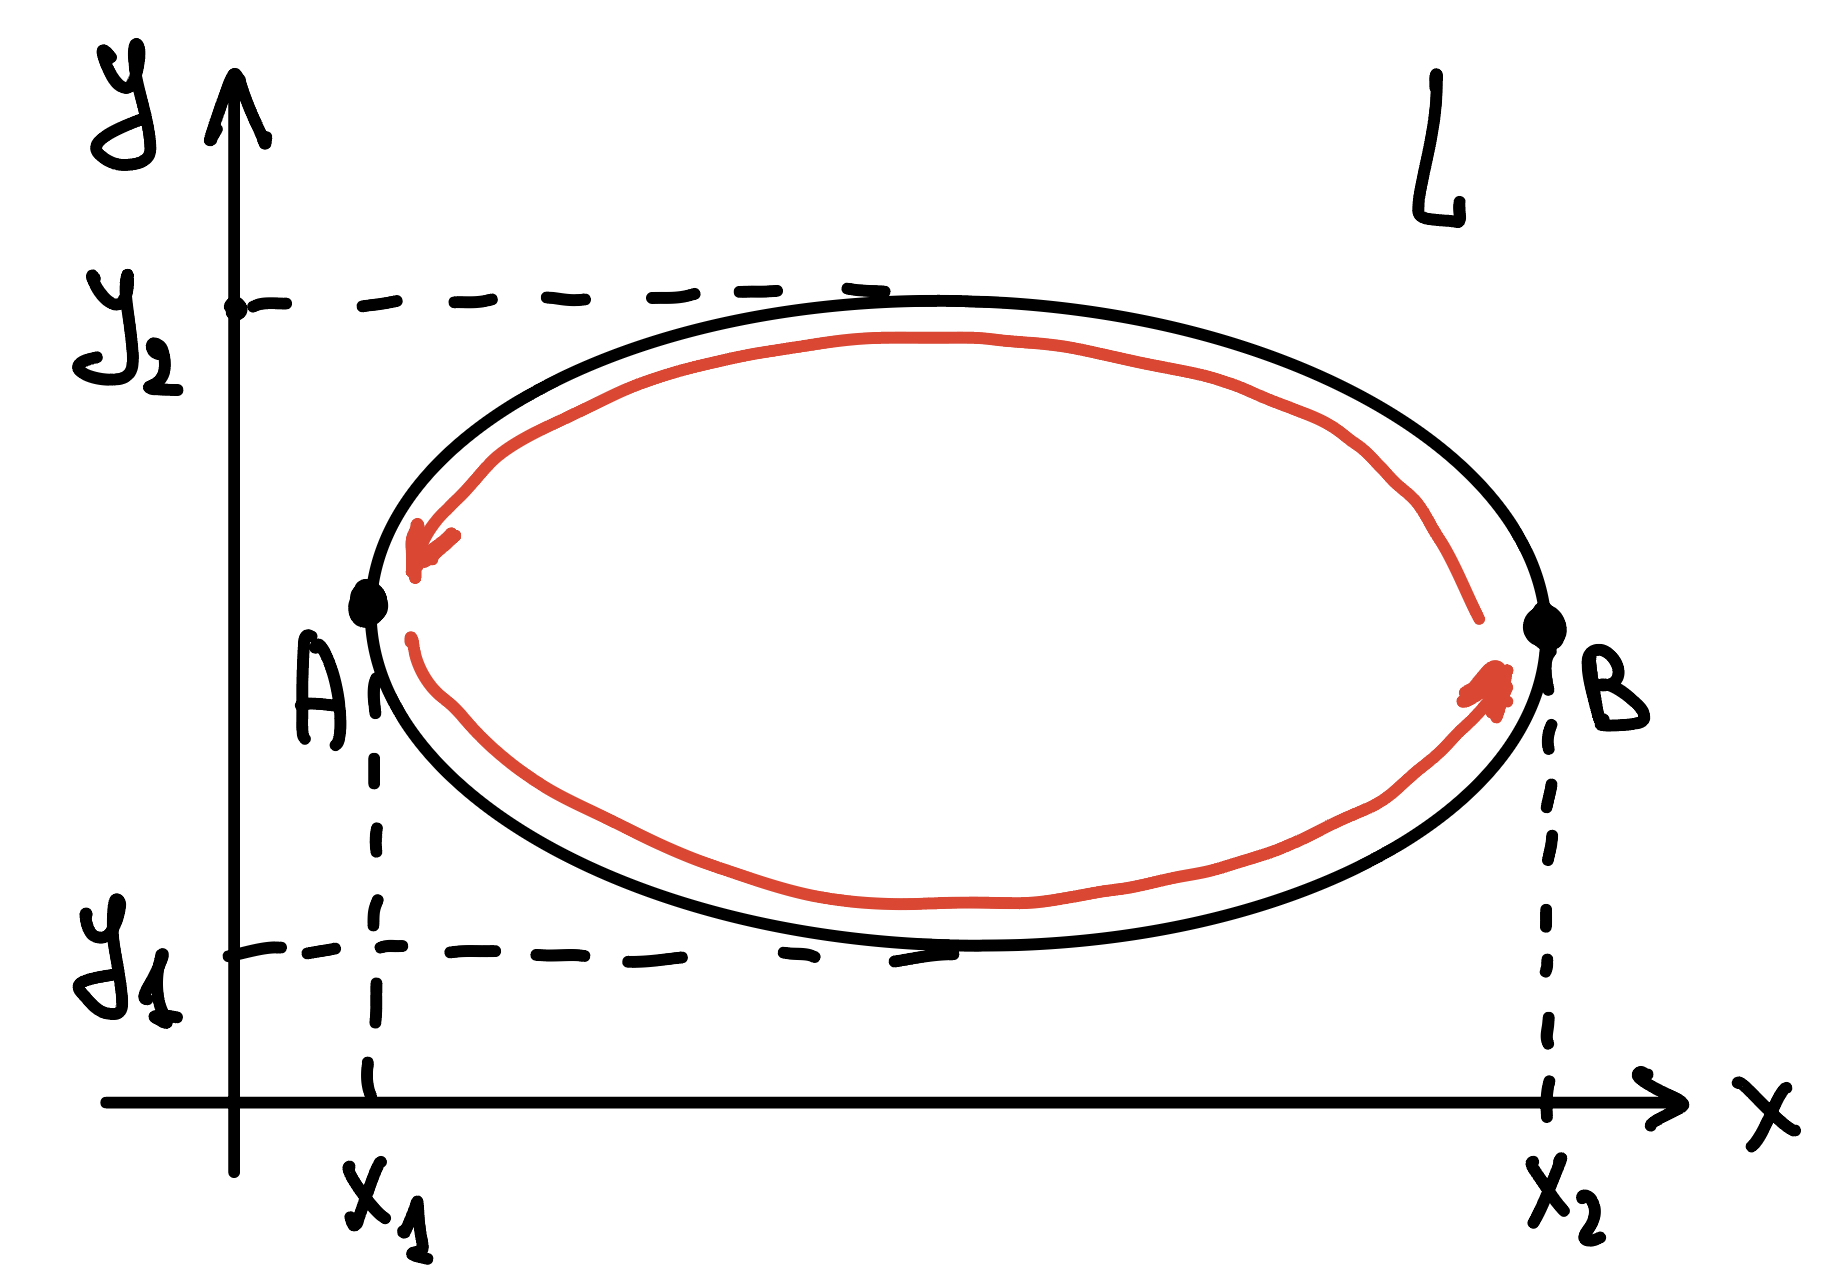
\includegraphics[scale=0.06]{pics/osn06_L.jpeg}

% Представим формулу Грина в покоординатной форме.

% \begin{proof}
% Введем ортонорм. Декартову сис. коорд.: $Oz \uparrow\uparrow \overline{k}$, $O_{xy}$ -- в плоскости $\pi$ и выбраны так, чтобы выполнялось "координатное свойство" на $D$
% $L: \{ x=x(t), ~ y = y(t) \}$ -- согласовано с направлением обхода.

% $\overline{a} = a_1(x,y,z)\overline{e}_1 + a_2(x,y,z)\overline{e}_2 + a_3(x,y,z)\overline{e}_3, ~ \overline{e}_3 = \overline{k}$, \\
% $rot(\overline{a}) = \dots + \left(\frac{\partial a_2}{\partial x} - \frac{\partial a_1}{\partial y} \right)\overline{e}_3 \Longrightarrow rot\left(\overline{a}, \overline{k}\right) = \frac{\partial a_2}{\partial x} - \frac{\partial a_1}{\partial y}$ в области $D$.

% $\overline{t} = \{x'(t), y'(t), 0\} \frac{1}{\sqrt{x'^2(t) + y'^2(t)}}$, $dl = \sqrt{x'^2(t) + y'^2(t)}dt \Longrightarrow
% \oint (\overline{a}, \overline{t})dl = \int_{t_1}^{t_2}(a_1(x,y,0)x'(t) + a_2(x,y,0)y'(t))dt = \oint\limits_{\mathcal{L}} (a_1(x,y,0)dx + a_2(x,y,0)dy)$

% $\iint\limits_{D}(\frac{\partial a_2}{\partial x} - \frac{\partial a_1}{\partial y})\bigg|_{z=0} dxdy$

% Пусть $P(x,y) = a_1(x,y,0), ~ Q(x, y) = a_2(x,y,0)$, тогда \textbf{Формула Грина} в покоординатной форме:
% $$\oint\limits_{L} (P(x,y)dx + Q(x,y)dy) = \iint\limits_{\overline{D}} (\frac{\partial Q}{\partial x} - \frac{\partial P}{\partial y}) dx dy$$
% \end{proof}

% Таким образом значение функции по третьей координате ($k$) не влияет на значение.
% Поэтому, не теряя общности, можем рассматривать функции, определенные только на плоскости: $a=\{P(x,y),Q(x,y)\}$.
% Докажем для этого прредставления для простой области.
% Пусть $L$ -- положительно ориентированная кусочно-гладкая замкнутая кривая на плоскости, а $D$ -- простая плоская область, ограниченная кривой $L$.
% Функции $P=P(x,y)$, $Q=Q(x,y)$ определены в области $D$ и имеют непрерывные частные производные $\frac{\partial P}{\partial y}, \frac{\partial Q}{\partial x}$.

% \begin{proof}
% Докажем по отдельности:

% \textbf{(1)}$ \oint\limits_{L}Pdx = \iint\limits_{\mathcal{D}}(-\frac{\partial P}{\partial y})dxdy$, 
% \textbf{(2)}$ \oint\limits_{L}Qdx = \iint\limits_{\mathcal{D}}(-\frac{\partial Q}{\partial y})dxdy$.

% $D: x_1 \leq x \leq x_2, ~ y_1(x) \leq y \leq y_2(x)$

% $(1) =\iint\limits_{\mathcal{D}}\frac{\partial P}{\partial y}dxdy = $
% $ -\int_{x_1}^{x_2}dx\int_{y_1(x)}^{y_2(x)} \left(\frac{\partial P}{\partial y} \right)dy = $
% $ -\int_{x_1}^{x_2}(P(x,y_2(x)) - P(x, y_1(x)))dx = -\int_{x_1}^{x_2}P(x, y_2(x))dx + \int_{x_1}^{x_2}P(x, y_1(x))dx = \int\limits_{\smile BA}P(x,y)dx + \int\limits_{\frown AB}P(x,y)dx$

% Аналогично, спроецируем D на $O_y$ - докажем вторую формулу.
% \end{proof}

\textbf{Формулировка}
Пусть $C$ -- положительно ориентированная кусочно-гладкая замкнутая кривая на плоскости, а $D$ -- область, ограниченная кривой $C$. 
Если 
%функция $P = P(x,y)$, $Q = Q(x,y)$ определены в области $D$ и имеют непрерывные частные производные
$\frac{\partial P}{\partial y}$, $\frac{\partial Q}{\partial x} \in \mathcal{C}(D)$, то

$\oint\limits_{C} P \,dx + Q \,dy = \iint\limits_{D} \left( \frac{\partial Q}{\partial x} - \frac{\partial P}{\partial y} \right) \,dx\,dy$

На символе интеграла часто рисуют окружность, чтобы подчеркнуть, что кривая $C$ замкнута.

\begin{proof}
\textbf{Доказательство ф. Грина для простой области}
%$D$ -- область, правильная в направлении $OY$, ограниченная замкнутой кривой $C$
\mathLet \ область $D$ -- криволинейная трапеция (область, правильная в направлении $OY$)
: $D = \{ (x,y)|a \le x \le b, y_1(x) \le y \le y_2(x) \}$

Для кривой $C$, ограничивающей область $D$ зададим направление обхода по часовой стрелке. Тогда:

$\iint\limits_{D} \frac{\partial P}{\partial y} \,dx\,dy = \int\limits_{a}^{b}dx \int\limits_{y_1(x)}^{y_2(x)} \frac{\partial P}{\partial y} \,dy = \int\limits_{a}^{b} (P(x,y_2(x)) - P(x,y_1(x))) \,dx =$
$= \int\limits_{a}^{b} P(x,y_2(x)) \,dx - \int\limits_{a}^{b} P(x,y_1(x)) \,dx \quad (1)$

Заметим, что оба полученных интеграла можно заменить криволинейными интегралами:
$\int\limits_{C_1} P(x,y) \,dx = -\int\limits_{-C_1} P(x,y) \,dx = -\int\limits_{a}^{b} P(x,y_1(x)) \,dx \quad (2)$
$\int\limits_{C_3} P(x,y) \,dx = \int\limits_{a}^{b} P(x,y_2(x)) \,dx \quad (3)$
Интеграл по $C_1$ берётся со знаком «минус», так как согласно ориентации контура $C$ направление обхода данной части -- от $b$ до $a$.

Криволинейные интегралы по $C_2$ и $C_4$ будут равны нулю, так как $x = \operatorname{const}$:
$\int\limits_{C_2} P(x,y) \,dx = 0 \quad (4)$
$\int\limits_{C_4} P(x,y) \,dx = 0 \quad (5)$

Заменим в (1) интегралы согласно (2) и (3), а также прибавим (4) и (5), равные нулю и поэтому не влияющие на значение выражения:\\
$\iint\limits_{D} \frac{\partial P}{\partial y} \,dx\,dy = \int\limits_{C_1} P(x,y) \,dx + \int\limits_{C_3} P(x,y) \,dx + \int\limits_{C_2} P(x,y) \,dx + \int\limits_{C_4} P(x,y) \,dx$

Так как обход по часовой стрелке при правой ориентации плоскости является отрицательным направлением, то сумма интегралов в правой части является криволинейным интегралом по замкнутой кривой $C$ в отрицательном направлении:
$\iint\limits_{D} \frac{\partial P}{\partial y} \,dx\,dy = -\int\limits_{C} P(x,y) \,dx \quad (6)$

Аналогично доказывается формула:\\
$\iint\limits_{D} \frac{\partial Q}{\partial x} \,dx\,dy = \int\limits_{C} Q(x,y) \,dy \quad (7)$
если в качестве области $D$ взять область, правильную в направлении $OX$.

Сложим (6) и (7):
$\int\limits_{C} P \,dx + Q \,dy = \iint\limits_{D} \left( \frac{\partial Q}{\partial x} - \frac{\partial P}{\partial y} \right) \,dx\,dy$
\end{proof}

% % -------- source --------
% \bigbreak
% [\cite[page 69-96]{replace_me}]